%\documentclass[spanish,a4paper]{article}
%\documentclass[a4paper,openright,11pt]{report}
\documentclass[11pt]{article}
\usepackage[utf8]{inputenc}
\usepackage[a4paper,margin=6em]{geometry}
\usepackage[spanish]{babel}

% Paquetes generales
\usepackage{amsmath}
\usepackage[utf8]{inputenc}%esto permite meter tildes sin el coso
\usepackage[spanish]{babel}
\usepackage{ifthen}
\usepackage{amssymb}
\usepackage{amsmath}
\usepackage{multicol}
\usepackage{multirow}
\usepackage[absolute]{textpos}
\usepackage{hyperref}
\usepackage{enumitem}
%\usepackage{graphicx}
\usepackage{caratula}
\usepackage{float}%este es el que acomoda bien las figures

\newcommand{\linea}{\noindent\rule{12cm}{0.4pt}}

%% **************************************************************************
%
%  Package 'caratula', version 0.5 (para componer caratulas de TPs del DC).
%
%  En caso de dudas, problemas o sugerencias sobre este package escribir a
%  Brian J. Cardiff (bcardif arroba gmail.com).
%  Nico Rosner (nrosner arroba dc.uba.ar).
%
% **************************************************************************

% ----- Informacion sobre el package para el sistema -----------------------

\NeedsTeXFormat{LaTeX2e}
\ProvidesPackage{caratula}[2013/08/04 v0.5 Para componer caratulas de TPs del DC]
\RequirePackage{ifthen}
\usepackage[pdftex]{graphicx}

% ----- Imprimir un mensajito al procesar un .tex que use este package -----

\typeout{Cargando package 'caratula' v0.5 (2013/08/04)}

% ----- Algunas variables --------------------------------------------------

\let\Materia\relax
\let\Submateria\relax
\let\Titulo\relax
\let\Subtitulo\relax
\let\Grupo\relax
\let\Fecha\relax
\let\Logoimagefile\relax
\newcommand{\LabelIntegrantes}{}
\newboolean{showLU}
\newboolean{showEntregas}
\newboolean{showDirectores}

% ----- Comandos para que el usuario defina las variables ------------------

\def\materia#1{\def\Materia{#1}}
\def\submateria#1{\def\Submateria{#1}}
\def\titulo#1{\def\Titulo{#1}}
\def\subtitulo#1{\def\Subtitulo{#1}}
\def\grupo#1{\def\Grupo{#1}}
\def\fecha#1{\def\Fecha{#1}}
\def\logoimagefile#1{\def\Logoimagefile{#1}}

% ----- Token list para los integrantes ------------------------------------

\newtoks\intlist\intlist={}

\newtoks\intlistSinLU\intlistSinLU={}

\newcounter{integrantesCount}
\setcounter{integrantesCount}{0}
\newtoks\intTabNombre\intTabNombre={}
\newtoks\intTabLU\intTabLU={}
\newtoks\intTabEmail\intTabEmail={}

\newcounter{directoresCount}
\setcounter{directoresCount}{0}
\newtoks\direcTabNombre\direcTabNombre={}
\newtoks\direcTabEmail\direcTabEmail={}

% ----- Comando para que el usuario agregue integrantes --------------------

\def\integrante#1#2#3{%
    \intlist=\expandafter{\the\intlist\rule{0pt}{1.2em}#1&#2&\tt #3\\[0.2em]}%
    \intlistSinLU=\expandafter{\the\intlistSinLU\rule{0pt}{1.2em}#1 & \tt #3\\[0.2em]}%
    %
    \ifthenelse{\value{integrantesCount} > 0}{%
        \intTabNombre=\expandafter{\the\intTabNombre & #1}%
        \intTabLU=\expandafter{\the\intTabLU & #2}%
        \intTabEmail=\expandafter{\the\intTabEmail & \tt #3}%
    }{
        \intTabNombre=\expandafter{\the\intTabNombre #1}%
        \intTabLU=\expandafter{\the\intTabLU #2}%
        \intTabEmail=\expandafter{\the\intTabEmail \tt #3}%
    }%
    \addtocounter{integrantesCount}{1}%
}

\def\director#1#2{%
    \ifthenelse{\value{directoresCount} > 0}{%
        \direcTabNombre=\expandafter{\the\direcTabNombre & #1}%
        \direcTabEmail=\expandafter{\the\direcTabEmail & \tt #2}%
    }{
        \direcTabNombre=\expandafter{\the\direcTabNombre #1}%
        \direcTabEmail=\expandafter{\the\direcTabEmail \tt #2}%
    }%
    \addtocounter{directoresCount}{1}%
}

% ----- Macro para generar la tabla de integrantes -------------------------

\newcommand{\tablaIntegrantes}{\ }

\newcommand{\tablaIntegrantesVertical}{%
\ifthenelse{\boolean{showLU}}{%
    \begin{tabular}[t]{| l @{\hspace{4ex}} c @{\hspace{4ex}} l|}
        \hline
        \multicolumn{1}{|c}{\rule{0pt}{1.2em} \LabelIntegrantes} & LU &  \multicolumn{1}{c|}{Correo electr\'onico} \\[0.2em]
        \hline \hline
        \the\intlist
        \hline
    \end{tabular}
}{
    \begin{tabular}[t]{| l @{\hspace{4ex}} @{\hspace{4ex}} l|}
        \hline
        \multicolumn{1}{|c}{\rule{0pt}{1.2em} \LabelIntegrantes} &  \multicolumn{1}{c|}{Correo electr\'onico} \\[0.2em]
        \hline \hline
        \the\intlistSinLU
        \hline
    \end{tabular}
    }%
}

\newcommand{\tablaIntegrantesHorizontal}{%
    \begin{tabular}[t]{ *{\value{integrantesCount}}{c} }
    \the\intTabNombre \\%
\ifthenelse{\boolean{showLU}}{
    \the\intTabLU \\%
}{}
    \the\intTabEmail %
    \end{tabular}%
}

\newcommand{\tablaDirectores}{%
\ifthenelse{\boolean{showDirectores}}{%
	\bigskip
	Directores

	\smallskip
    \begin{tabular}[t]{ *{\value{directoresCount}}{c} }
    \the\direcTabNombre \\%
    \the\direcTabEmail %
    \end{tabular}%
}{}%
}

\newcommand{\tablaEntregas}{%
\ifthenelse{\boolean{showEntregas}}{%
  \bigskip%
  \begin{tabular}[t]{|l p{3.5cm} p{1.5cm}|}%
  \hline%
  \rule{0pt}{1.2em} Instancia & Docente & Nota \\[0.2em] %
  \hline%
  \hline%
  \rule{0pt}{1.2em} Primera entrega & & \\[0.2em] %
  \hline%
  \rule{0pt}{1.2em} Segunda entrega & & \\[0.2em] %
  \hline%
  \end{tabular}%
}{}%
}

% ----- Codigo para manejo de errores --------------------------------------

\def\se{\let\ifsetuperror\iftrue}
\def\ifsetuperror{%
    \let\ifsetuperror\iffalse
    \ifx\Materia\relax\se\errhelp={Te olvidaste de proveer una \materia{}.}\fi
    \ifx\Titulo\relax\se\errhelp={Te olvidaste de proveer un \titulo{}.}\fi
    \edef\mlist{\the\intlist}\ifx\mlist\empty\se%
    \errhelp={Tenes que proveer al menos un \integrante{nombre}{lu}{email}.}\fi
    \expandafter\ifsetuperror}

\def\aftermaketitle{%
  \setcounter{page}{1}
}

% ----- \maketitletxt correspondiente a la versi�n v0.2.1 (texto v0.2 + fecha ) ---------

\def\maketitletxt{%
    \ifsetuperror\errmessage{Faltan datos de la caratula! Ingresar 'h' para mas informacion.}\fi
    \thispagestyle{empty}
    \begin{center}
    \vspace*{\stretch{2}}
    {\LARGE\textbf{\Materia}}\\[1em]
    \ifx\Submateria\relax\else{\Large \Submateria}\\[0.5em]\fi
    \ifx\Fecha\relax\else{\Large \Fecha}\\[0.5em]\fi
    \par\vspace{\stretch{1}}
    {\large Departamento de Computaci\'on}\\[0.5em]
    {\large Facultad de Ciencias Exactas y Naturales}\\[0.5em]
    {\large Universidad de Buenos Aires}
    \par\vspace{\stretch{3}}
    {\Large \textbf{\Titulo}}\\[0.8em]
    {\Large \Subtitulo}
    \par\vspace{\stretch{3}}
    \ifx\Grupo\relax\else\textbf{\Grupo}\par\bigskip\fi
    \tablaIntegrantes
    \end{center}
    \vspace*{\stretch{3}}
    \newpage\aftermaketitle}

% ----- \maketitletxtlogo correspondiente v0.2.1 (texto con fecha y logo) ---------

\def\maketitletxtlogo{%
    \ifsetuperror\errmessage{Faltan datos de la caratula! Ingresar 'h' para mas informacion.}\fi
    \thispagestyle{empty}
    \begin{center}
    \ifx\Logoimagefile\relax\else\includegraphics{\Logoimagefile}\fi \hfill 
\includegraphics{logo_dc.jpg}\\[1em]
    \vspace*{\stretch{2}}
    {\LARGE\textbf{\Materia}}\\[1em]
    \ifx\Submateria\relax\else{\Large \Submateria}\\[0.5em]\fi
    \ifx\Fecha\relax\else{\large \Fecha}\\[0.5em]\fi
    \par\vspace{\stretch{1}}
    {\large Departamento de Computaci\'on}\\[0.5em]
    {\large Facultad de Ciencias Exactas y Naturales}\\[0.5em]
    {\large Universidad de Buenos Aires}
    \par\vspace{\stretch{3}}
    {\Large \textbf{\Titulo}}\\[0.8em]
    {\Large \Subtitulo}
    \par\vspace{\stretch{3}}
    \ifx\Grupo\relax\else\textbf{\Grupo}\par\bigskip\fi
    \tablaIntegrantes
    \end{center}
    \vspace*{\stretch{4}}
    \newpage\aftermaketitle}

% ----- \maketitlegraf correspondiente a la versi�n v0.3 (gr�fica) -------------

\def\maketitlegraf{%
    \ifsetuperror\errmessage{Faltan datos de la caratula! Ingresar 'h' para mas informacion.}\fi
%
    \thispagestyle{empty}

    \ifx\Logoimagefile\relax\else\includegraphics{\Logoimagefile}\fi \hfill 
\includegraphics{logo_dc.jpg}

    \vspace*{.06 \textheight}

    \noindent \textbf{\huge \Titulo}  \medskip \\
    \ifx\Subtitulo\relax\else\noindent\textbf{\large \Subtitulo} \\ \fi%
    \noindent \rule{\textwidth}{1 pt}

    {\noindent\large\Fecha \hspace*\fill \Materia} \\
    \ifx\Submateria\relax\else{\noindent \hspace*\fill \Submateria}\fi%

    \medskip%
    \begin{center}
        \ifx\Grupo\relax\else\textbf{\Grupo}\par\bigskip\fi
        \tablaIntegrantes

        \tablaDirectores

        \tablaEntregas
    \end{center}%
    \vfill%
%
    \begin{minipage}[t]{\textwidth}
        \begin{minipage}[t]{.55 \textwidth}
            
\includegraphics{logo_uba.jpg}
        \end{minipage}%%
        \begin{minipage}[b]{.45 \textwidth}
            \textbf{\textsf{Facultad de Ciencias Exactas y Naturales}} \\
            \textsf{Universidad de Buenos Aires} \\
            {\scriptsize %
            Ciudad Universitaria - (Pabell\'on I/Planta Baja) \\
                Intendente G\"uiraldes 2160 - C1428EGA \\
            Ciudad Aut\'onoma de Buenos Aires - Rep. Argentina \\
                Tel/Fax: (54 11) 4576-3359 \\
            http://www.fcen.uba.ar \\
            }
        \end{minipage}
    \end{minipage}%
%
    \newpage\aftermaketitle}

% ----- Reemplazamos el comando \maketitle de LaTeX con el nuestro ---------
\renewcommand{\maketitle}{\maketitlegraf}

% ----- Dependiendo de las opciones ---------
%
% opciones:
%   txt     : caratula solo texto.
%   txtlogo : caratula txt con logo del DC y del grupo (opcional).
%   graf    : (default) caratula grafica con logo del DC, UBA y del grupo (opcional).
%
\@makeother\*% some package redefined it as a letter (as color.sty)
%
% Layout general de la caratula
%
\DeclareOption{txt}{\renewcommand{\maketitle}{\maketitletxt}}
\DeclareOption{txtlogo}{\renewcommand{\maketitle}{\maketitletxtlogo}}
\DeclareOption{graf}{\renewcommand{\maketitle}{\maketitlegraf}}
%
% Etiqueta Autores o Integrantes
%
\DeclareOption{integrante}{\renewcommand{\LabelIntegrantes}{Integrante}}
\DeclareOption{autor}{\renewcommand{\LabelIntegrantes}{Autor}}
%
% Formato tabla de integrantes
%
\DeclareOption{intVert}{\renewcommand{\tablaIntegrantes}{\tablaIntegrantesVertical}}
\DeclareOption{intHoriz}{\renewcommand{\tablaIntegrantes}{\tablaIntegrantesHorizontal}}
\DeclareOption{conLU}{\setboolean{showLU}{true}}
\DeclareOption{sinLU}{\setboolean{showLU}{false}}
\DeclareOption{conEntregas}{\setboolean{showEntregas}{true}}
\DeclareOption{sinEntregas}{\setboolean{showEntregas}{false}}
\DeclareOption{showDirectores}{\setboolean{showDirectores}{true}}
\DeclareOption{hideDirectores}{\setboolean{showDirectores}{false}}
%
% Opciones predeterminadas
%
\ExecuteOptions{intVert}%
\ExecuteOptions{graf}%
\ExecuteOptions{integrante}%
\ExecuteOptions{conLU}%
\ExecuteOptions{hideDirectores}%
\ExecuteOptions{sinEntregas}%
%
\ProcessOptions\relax

\begin{document}


\titulo{Trabajo Pr\'{a}ctico: Scheduling}
\subtitulo{}

\fecha{\today}

\materia{Sistemas Operativos}
\grupo{}

\integrante{Arribas, Joaquín}{702/13}{joacoarribas@hotmail.com}
\integrante{Lebrero, Ignacio}{702/13}{nachitou@hotmail.com}
\integrante{Vázquez, Jésica}{702/13}{jesis\_93@hotmail.com}

\maketitle

\thispagestyle{empty}
\vspace{3cm}
\tableofcontents
\newpage
\vfill

\begin{abstract}
Con el crecimiento de los sistemas operativos y la capacidad de hardware para soportar varios procesos, surgen nuevos desafios a la hora de diseñar dichos sistemas. Uno de ellos es la organizacion de los procesos o $scheduling$, pero...¿hay una manera optima de hacerlo?, la respuesta es que depende cual sea la finalidad del sistema, Para esto existen muchos criterios bajo los cuales pueden ser organizados los procesos. 
 En este trabajo se implementaron distintas simulaciones interactivas entre tareas. A su vez se implementaron distintas clases de scheduling para interactuar 
 con las tareas creadas, y dichas interacciones se representaron de manera gráfica.
  Hare que no se hablar, i know that feling bro.
\end{abstract}

\newpage

\section{Ejercicio 1}

El ejercicio consiste en implementar una tarea llamada \textbf{TaskConsola}, que simule una tarea que realiza llamadas bloqueantes. La tarea 
recibe por parámetro la cantidad de llamadas bloqueantes que debe realizar, y un intervalo que determina un máximo y un mínimo para la duración 
de cada una. Dicha duración es generada de manera pseudoaleatoria.

Para resolver el ejercicio creamos una función llamada \textbf{generate} que se encarga de realizar la simulación de la tarea. Genera una $semilla$ utilizando la función 
\textbf{time} y luego, para cada llamada bloqueante, genera el tiempo usando la función \textbf{rand\_r}. Para cada valor de la semilla 
se genera un valor pseudoaleatorio al cual se lo fuerza a caer en el intervalo pasado por parametro, tomandole módulo la distancia entre el máximo y 
el mínimo, y luego sumandole el mínimo. Una vez calculado el tiempo, se hace la llamada al uso del dispositivo de I/O.

Ejemplo: 

      \begin{figure}[H]
        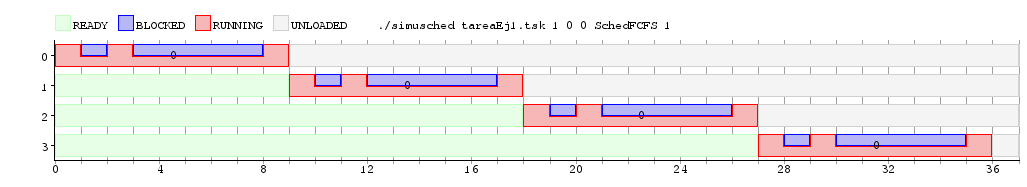
\includegraphics[scale=0.5]{ejercicio1}
      \end{figure}

El gráfico esta corriendo un lote de 4 tareas de tipo \textbf{TaskConsola}. El algoritmo de $scheduling$ utilizado para representar la interacción 
entre las tareas es \textbf{First Come, First Served}. La cantidad de llamadas bloqueantes son 2 y el intervalo de 
tiempo para cada llamada es entre 2 y 6. Podemos observar como efectivamente la duración de cada llamada bloqueante pertenece a ese 
intervalo

\newpage

\section{Ejercicio 2}

El ejercicio consiste en simular la situación que enfrenta nuestro querido amigo Rolando, el cual quiere correr un algoritmo a la vez que escucha 
música y consume drogas. El algoritmo que corre hace un uso intensivo del cpu por 100 ciclos, mientras que la música y el internet realizan una 
cantidad determinada de llamadas bloqueantes. La música realiza 20 y el internet 25, cada una de duración variable entre 2 y 4 ciclos. La manera 
de generar la duración pseudoaleatoria de los ciclos de las llamadas bloqueantes fue la misma que la utilizada en el ejercicio previo, a través 
de la funcion \textbf{generate}. El algoritmo de $scheduling$ utilizado para este ejercicio fue \textbf{First Come, First Served}.

Ejemplos:

\section{Ejercicio 3}

\newpage 

\section{Ejercicio 4}

En este ejercicio completamos la implentación del scheduler \textit{Round-Robin}. Éste consiste en asignarle un quantum determinado a cada tarea. Cada núcleo puede, o no, tener quantum distintos. 

\subsection{Elección de estructuras}

Para la implementación del scheduler utilizamos una cola con las tareas que están en estado LISTAS, y almacenamos en un vector aquellas que están BLOQUEADAS. Además, cada núcleo conoce cuál es la tarea que está CORRIENDO, y cuántos ciclos lleva, con lo cual, dado que tiene un quantum determinado, calcula en qué momento debe desalojarla y darle el procesador a la próxima tarea.
Hay una única cola de tareas, en decir, se permite la migración de núcleos, ya que el scheduler desencola la primer tarea en estado LISTA y le asigna el núcleo que esté libre en ese momento. 

\newpage

\section{Ejercicio 5}

En esta sección evaluaremos el rendimiento del scheduler \textit{Round-Robin} según el tiempo de latencia, el waiting-time (tiempo que el proceso está en estado READY), y el tiempo total de ejecución. Utilizaremos un lote de tareas con una de tipo \textbf{TaskCPU} de 50 ciclos, y dos \textbf{TaskConsola2} que hacen 5 llamadas bloqueantes, cada una de ella de duración de 3 ciclos. 
Los cálculos de los cuadros están hechos sobre los datos de la simulación. \\

%./simusched tareaEj5.tsk 1 2 0 SchedRR 1 2 CON ESTE COMANDO GENERE LA IMAGEN, LO DEJO PAL MAKEFILE 

\subsection{Análisis de \textit{Round-Robin} para distintos quantum}
\begin{enumerate}
\item \textbf{Round-Robin con quantum 2}

      \begin{figure}[H]
        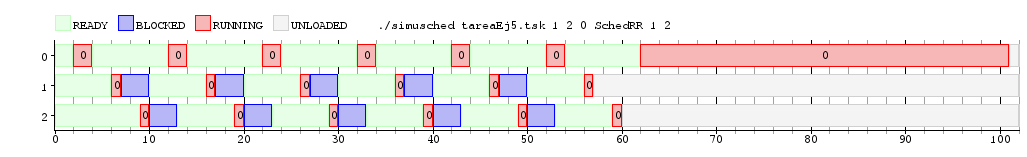
\includegraphics[scale=0.5]{Ej5q2}
        \caption{Simulación SchedRR quantum 2}
      \end{figure}

%TABLA PARA QUANTUM 2
\begin{table}[htb]
%\begin{center}
\centering
\begin{tabular}{| l | l | l | l |}
\hline
" " & Task0 & Task1 & Task2 \\
\hline \hline
Latencia & 2 & 6 & 9 \\ \hline
Waiting Time & 50 & 41 & 44 \\ \hline
Tiempo de Ejecución & 100 & 55 & 60 \\ \hline
\end{tabular}
\caption{cálculos con quantum 2}
%\end{center}
\end{table}

En este caso se observa que las 3 tarea tienen un tiempo de espera elevado con respecto al tiempo de ejecución total. La \textbf{Task0} espera durante el 50\% del tiempo, mientras que las \textbf{Task1} y \textbf{Task2} esperan aproximadamente 74,5\% y 73,3\% respectivamente. Por otro lado, la latencia de los procesos es baja con respecto a la cantidad de ciclos que le lleva terminar de ejecutarse. 

\item \textbf{Round-Robin con quantum 10}

      \begin{figure}[H]
        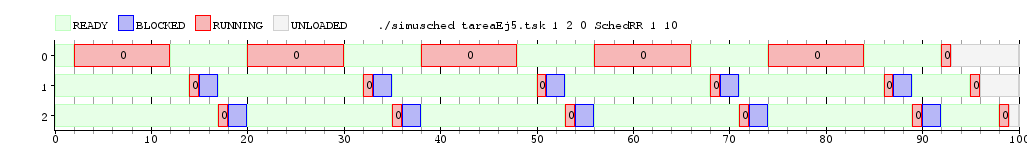
\includegraphics[scale=0.5]{Ej5q10}
        \caption{Simulación SchedRR quantum 10}
      \end{figure}

%TABLA PARA QUANTUM 10
\begin{table}[htb]
%\begin{center}
\centering
\begin{tabular}{| l | l | l | l |}
\hline
" " & Task0 & Task1 & Task2 \\
\hline \hline
Latencia & 2 & 14 & 17 \\ \hline
Waiting Time & 42 & 80 & 83 \\ \hline
Tiempo de Ejecución & 93 & 96 & 99 \\ \hline
\end{tabular}
\caption{cálculos con quantum 10}
%\end{center}
\end{table}

Para el scheduler con quantum 10, se observa una mejora con respecto al tiempo de espera de la \textbf{Task 0}, disminuyendo el porcentaje a aproximadamente el 45,2\%, sin embargo, las otras dos tareas elevaron su tiempo de espera a alrededor del 83\%. Al igual que en el caso anterior, la latencia continúa siendo relativamente baja.

\item \textbf{Round-Robin con quantum 50}

      \begin{figure}[H]
        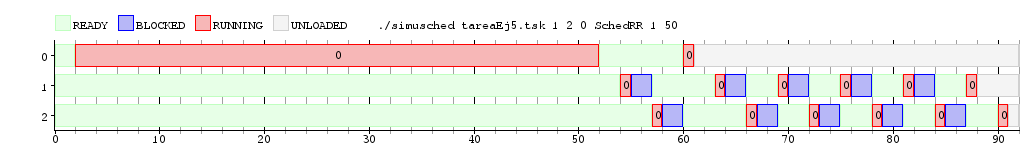
\includegraphics[scale=0.5]{Ej5q50}
        \caption{Simulación SchedRR quantum 50}
      \end{figure}

%TABLA PARA QUANTUM 50
\begin{table}[htb]
%\begin{center}
\centering
\begin{tabular}{| l | l | l | l |}
\hline
" " & Task0 & Task1 & Task2 \\
\hline \hline
Latencia & 2 & 54 & 57 \\ \hline
Waiting Time & 10 & 72 & 75 \\ \hline
Tiempo de Ejecución & 61 & 88 & 91 \\ \hline
\end{tabular}
\caption{cálculos con quantum 50}
%\end{center}
\end{table}

En este caso, el porcentaje de tiempo de espera de la \textbf{Task 0} disminuye notablemente a un 16,4\%, y los tiempos de espera de las tareas restantes están alrededor de 82\%, porcentaje similar al caso del scheduler de quantum 10. Sin embargo, como en este caso se le asigna un quantum elevado a la primer tarea, el tiempo de latencia de las \textbf{Task 1} y \textbf{Task 2} ahora es de 54 y 57 ciclos respectivamente. 
\end{enumerate}

\subsection{Conclusión}
HARE LOCO

\newpage

\section{Ejercicio 6}

      \begin{figure}[H]
        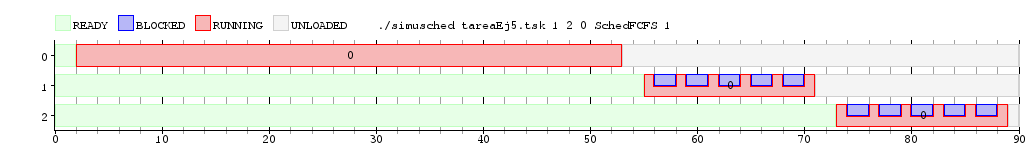
\includegraphics[scale=0.5]{Ej6}
        \caption{Simulación SchedFCFS quantum 2}
      \end{figure}


\end{document}

